\chapter{Evolution and thermodynamics of black holes}
\label{s:evo}

\minitoc

\section{Introduction}

This chapter is in a draft stage.

\section{Towards the first law of black hole dynamics}

\subsection{Mass variation formula for Kerr black holes}

In this section, we assume 4-dimensional general relativity.
Let us consider an initially isolated Kerr black hole of mass and spin parameters $(m,a)$
that is perturbed by the arrival of some external body or some gravitational
radiation. After some transitory dynamical regime (e.g. absorption of the
external body and emission of gravitational waves), the black hole relaxes
to a new equilibrium configuration. According to the
no-hair theorem (Property~\ref{p:sta:no-hair_thm}, Sec.~\ref{s:sta:no-hair}),
the final state has to be a Kerr black hole, of
parameters $(m+\D m, a+\D a)$ say. All global properties of the black
hole (cf. Sec.~\ref{s:ker:global_quantities})
are changed accordingly and we are going to express the change in
the Komar mass $M = m$ [Eq.~(\ref{e:ker:M_m})] in terms of the change in
the area $A = 8 \pi m (m + \sqrt{m^2-a^2})$ [Eq.~(\ref{e:ker:A_a_m})]
and in the angular momentum $J = a m$ [Eq.~(\ref{e:ker:J_am})].

Rewriting Eq.~(\ref{e:ker:A_a_m}) as $A = 8 \pi (M^2 + \sqrt{M^4 - J^2})$
and differentiating, we get
\[
\frac{1}{8\pi} \, \D A =  2 M\,  \D M + \frac{2M^3}{\sqrt{M^4-J^2}}\, \D M
    - \frac{J}{\sqrt{M^4-J^2}}\, \D J ,
\]
or equivalently
\[
    \D M = \frac{1}{8\pi}
\underbrace{\frac{\sqrt{M^4-J^2}}{2M(M^2+\sqrt{M^4-J^2})}}_{\kappa} \, \D A
+ \underbrace{\frac{J}{2M(M^2+\sqrt{M^4-J^2})}}_{\Omega_{\Hor}} \, \D J  ,
\]
where the identifications of the black hole's surface gravity $\kappa$ and
rotation velocity $\Omega_{\Hor}$ result from Eqs.~(\ref{e:ker:kappa_m_a})
and (\ref{e:ker:def_OmegaH}) respectively. Hence we get
\be \label{e:evo:mass_variation}
    \encadre{ \D M = \frac{\kappa}{8\pi} \, \D A + \Omega_{\Hor} \, \D J } .
\ee
\begin{remark}
The mass variation formula (\ref{e:evo:mass_variation}) is \emph{not}
the mere differential of the Smarr formula (\ref{e:ker:Smarr}):
$ M =  \kappa A/(4\pi) + 2 \Omega_{\Hor} J$.
Indeed, differentiating the latter yields
\[
    \D M = \frac{\kappa}{4\pi} \, \D A +  \frac{A}{4\pi} \, \D \kappa
        + 2 \Omega_{\Hor} \, \D J  + 2 J \, \D\Omega_{\Hor} .
\]
Since $\kappa$ and $\Omega_{\Hor}$ depend on $m$ and $a$ [Eqs.~(\ref{e:ker:kappa_m_a})
and (\ref{e:ker:def_OmegaH})], one has
$\D\kappa \neq 0$ and $\D\Omega_{\Hor}\neq 0$ when moving
from $(m,a)$ to $(m+\D m, a+\D a)$.
If one were (wrongly) assuming $\D\kappa = 0$ and $\D\Omega_{\Hor} = 0$, one would
be wrong by a factor of 2 in recovering the right-hand side of
Eq.~(\ref{e:evo:mass_variation}).
\end{remark}

\subsection{General mass variation formula} \label{s:evo:gen_mass_variation}

The mass variation formula (\ref{e:evo:mass_variation}) can be derived in
a more general framework, without assuming that it describes changes between
two nearby Kerr solutions \cite{BardeCH73,Carte79} and without restricting
the spacetime dimension to 4. It even holds
for other gravity theories than general relativity, more specifically
for any theory based on a diffeomorphism-covariant lagrangian; see Wald's review
article~\cite{Wald01} for details.

Here we establish the mass variation formula for two nearby black hole
equilibrium configurations, from integral mass formulas obtained in Chap.~\ref{s:sta}.
More precisely, we consider a stationary spacetime $(\M,\w{g})$ that contains
a black hole and a ``nearby'' black hole spacetime $(\M,\w{g}+\delta\w{g})$ that has the
same symmetries (stationarity and possible axisymmetries) as $(\M,\w{g})$.
We shall call $(\M,\w{g}+\delta\w{g})$ the \defin{perturbed spacetime}\index{perturbed!spacetime},
although we do not require that $(\M,\w{g}+\delta\w{g})$ is obtained from
$(\M,\w{g})$ by some specific physical perturbation.
Note that the same manifold $\M$ is used for both spacetimes.
There is no loss of generality in doing so, since the perturbed manifold
must be diffeomorphic to the original one, which allows one to
identify the two manifolds. In particular, both manifolds have the same
topology, since one would not qualify as ``nearby'' a manifold with a distinct topology.


\begin{prop}[mass variation formula for generic black holes]
\label{p:evo:first_law_gen}
Let $(\M,\w{g})$ be a $n$-dimensional stationary spacetime (stationary
Killing vector $\w{\xi}$) that contains a black
hole, the event horizon of which has $K \geq 1$ connected components
$\Hor_{1}$, $\ldots$, $\Hor_{K}$.
We shall assume that each $\Hor_{k}$ is a Killing horizon
with respect to a Killing vector $\w{\chi}_{k}$.
This is guaranteed with $\w{\chi}_k = \w{\xi}$
if $\Hor_{k}$ is non-rotating ($\w{\xi}$ null on all $\Hor_{k}$;
Property~\ref{p:sta:H_Killing_hor_xi_null}), while if
$\Hor_{k}$ is rotating ($\w{\xi}$ spacelike on some parts of $\Hor_{k}$),
this holds under the hypotheses of the strong rigidity theorem
(Property~\ref{p:sta:strong_rigidity_thm}),
with
\be \label{e:evo:chi_k}
\w{\chi}_{k} = \w{\xi} + \sum_{i=1}^{L_{k}} \Omega^{(i)}_{\Hor_k} \w{\eta}_{\Hor_k(i)},
\ee
where $1 \leq L_k \leq [(n-1)/2]$,
the $\Omega^{(i)}_{\Hor_k}$'s are constants and
the $\w{\eta}_{\Hor_k(i)}$'s are axisymmetric Killing vectors
(Property~\ref{p:sta:axisymmetry_BH}).
We shall encompass both the non-rotating case and the rotating one by allowing
$L_k$ to take the value $0$ in Eq.~(\ref{e:evo:chi_k}) to
recover $\w{\chi}_k = \w{\xi}$  if $\Hor_k$ is non-rotating.
Let $J_{\Hor_{k}(i)}$ be the Komar angular momentum with respect to
$\w{\eta}_{\Hor_k(i)}$ over any cross-section of $\Hor_{k}$
[Eq.~(\ref{e:sta:def_Komar_J})].
Being a non-expanding horizon, each
$\Hor_{k}$ has a well defined area $A_{k}$ (Property~\ref{p:neh:invariance_area}).
Let $\kappa_{k}$ be the surface gravity of $\Hor_{k}$, i.e.
the coefficient such that
$\wnab_{\w{\chi}_{k}}\w{\chi}_{k} =  \kappa_{k} \w{\chi}_{k}$
 on $\Hor_{k}$ [cf. Eq.~(\ref{e:neh:xi_nab_xi_kappa})].
Let us assume that the null dominance condition (\ref{e:neh:null_dominant_cond}) is fulfilled
on $\Hor_{k}$; by the zeroth law of black hole dynamics (Property~\ref{p:neh:zeroth_law}), this
implies that $\kappa_{k}$ is constant.
Let $(\M,\w{g}+\delta\w{g})$ be a nearby stationary spacetime sharing the same characteristics.
The change $\delta M_\infty$ of the Komar at infinity between the two spacetimes
(cf. Property~\ref{p:sta:Komar_mass_inf})
is related to the changes $\delta A_k$ in the areas and to the changes
$\delta J_{\Hor_{k}(i)}$ in the Komar angular momenta by
\bea
    \delta  M_\infty & = & \sum_{k = 1}^K
    \left(
    \frac{\kappa_{k}}{8\pi}\, \delta A_k
    +  \sum_{i=1}^{L_{k}} \Omega^{(i)}_{\Hor_k} \, \delta J_{\Hor_{k}(i)} \right) \nonumber \\
    & & + \frac{1}{16\pi}
    \int_{\Sigma} G^{\mu\nu} \delta g_{\mu\nu} \, \xi_\rho \D V^\rho
        - \frac{1}{8\pi} \,
   \delta  \int_{\Sigma} G_{\mu\nu} \, \xi^\mu \D V^\nu ,  \label{e:evo:mass_variation_gal}
\eea
where $\Sigma$ is any asymptotically flat spacelike hypersurface, the inner boundary
of which is a cross-section of the event horizon, i.e. some union of cross-sections
of the connected components $\Hor_{k}$,
$\w{G}$ is the Einstein tensor of $\w{g}$
and $\D\w{V}$
is the normal volume element vector of $\Sigma$, as defined by Eq.~(\ref{e:sta:normal_vol_element}).
\end{prop}

\begin{proof}
We may consider that the black hole event horizon $\Hor$ is the same
hypersurface in both spacetimes $(\M,\w{g})$ and $(\M,\w{g}+\delta\w{g})$. If the horizons would differ, we could find a diffeomorphism
$\M\to\M$ that would map the original horizon to the perturbed spacetime's horizon.
Similarly, there is no loss of generality in considering that the Killing vectors
$\w{\xi}$ and $\w{\eta}_{\Hor_k(i)}$ generating the stationarity and axisymmetries are identical, as vector fields on $\M$:
\be \label{e:evo:delta_xi_eta}
    \delta\w{\xi} = 0 \qand \delta \w{\eta}_{\Hor_k(i)} = 0 .
\ee
 This amounts to identifying the orbits
of the isometry group actions in the two spacetimes. Given that $\Hor$ is globally invariant by these
group actions, this requirement is compatible with the identification of $\Hor$ in both spacetimes.
Let us introduce the short-hand notation $\w{h} := \delta\w{g}$, or in index notation
$h_{\alpha\beta} = \delta g_{\alpha\beta}$. In all what follows, indices will be raised or lowered
with the unperturbed metric $\w{g}$. In particular, $h^{\alpha\beta} := g^{\alpha\mu} g^{\beta\nu} h_{\mu\nu}$.
Note that $h^{\alpha\beta} \neq \delta g^{\alpha\beta}$. Actually, by variation of the
identity $g^{\alpha\mu} g_{\mu\beta} = \delta^\alpha_{\ \, \beta}$, one gets
$\delta g^{\alpha\beta} = - h^{\alpha\beta}$.
The starting point for proving (\ref{e:evo:mass_variation_gal})
is the variation of the generalized Smarr formula (\ref{e:sta:Smarr_M_infty_R}):
\bea
 \frac{2(n- 3)}{n - 2} \delta  M_\infty& = &\sum_{k = 1}^K
    \left[
    \frac{1}{4\pi} \left( A_k\,  \delta \kappa_{k}  + \kappa_k \, \delta A_k \right)
    + 2  \sum_{i=1}^{L_{k}} \left( J_{\Hor_{k}(i)} \, \delta \Omega^{(i)}_{\Hor_k}
    + \Omega^{(i)}_{\Hor_k} \, \delta J_{\Hor_{k}(i)} \right) \right] \nonumber \\
    & &
     - \frac{1}{4\pi} \delta \int_{\Sigma} R_{\mu\nu} \, \xi^\nu \D V^\mu ,
\eea
where $\Sigma$ is any asymptotically flat spacelike hypersurface, the inner boundary
of which is a cross-section of the event horizon, i.e. some union of cross-sections $\Sp_k$
of the connected components $\Hor_{k}$ and $\D V^\mu$ is the normal volume element vector
of $\Sigma$ defined by Eq.~(\ref{e:sta:normal_vol_element}).
Let us start by evaluating the term $A_k\,  \delta \kappa_{k}$ in the above formula.
For the sake of brevity, let us drop the index $k$ in what follows, given that
we temporarily focuss on a single connected component $\Hor_k$ of the event horizon $\Hor$.
The surface gravity $\kappa$ $(= \kappa_k)$ is given by Eq.~(\ref{e:neh:dxi2_kappa}):
$2\kappa = k^\mu \partial_\mu(\chi_\nu \chi^\nu)$, where $\w{\chi}$ ($ = \w{\chi}_k$) is the Killing vector
normal to the Killing horizon $\Hor_k$ and $\w{k}$ is a null vector field defined on $\Hor_k$,
transverse to $\Hor_k$, normal
to the cross-section $\Sp_k = \Hor_k \cap \Sigma$
and normalized by $\w{\chi}\cdot\w{k}=-1$.
Note that the pair
$(\w{\chi},\w{k})$ is a null basis of the normal plane $T^\perp_p \Sp_k$
at each point $p\in\Sp_k$,
$\w{\chi}$ playing the role of the vector $\wl$ in Fig.~\ref{f:def:TS_ortho}.
Varying the above expression of $\kappa$ yields
\bea
    2 \delta \kappa & = & \delta k^\mu \partial_\mu ( \chi_\nu \chi^\nu )
    + k^\mu \partial_\mu \left( \delta\chi_\nu \, \chi^\nu
        + \chi_\nu \, \delta \chi^\nu \right) \nonumber \\
        & = & \delta k^\mu \nabla_\mu ( \chi_\nu \chi^\nu )
    +  k^\mu \nabla_\mu \left( \delta\chi_\nu \, \chi^\nu
        + \chi_\nu \, \delta \chi^\nu \right)  \nonumber \\
        & = & 2 \delta k^\mu  \chi^\nu \nabla_\mu  \chi_\nu
        + k^\mu \left( \chi^\nu \nabla_\mu \delta\chi_\nu
         + \delta\chi_\nu  \nabla_\mu \chi^\nu
         + \delta \chi^\nu  \nabla_\mu \chi_\nu  +  \chi_\nu \nabla_\mu \delta \chi^\nu
        \right)  \nonumber \\
    & = &  2 \delta k^\mu  \chi^\nu \nabla_\mu  \chi_\nu + k^\mu \left[
        \chi^\nu ( \nabla_\mu \delta\chi_\nu + \nabla_\nu \delta \chi_\mu )
        + 2 \delta\chi_\nu \nabla_\mu \chi^\nu
        + \delta \chi^\nu \nabla_\mu \chi_\nu + \chi_\nu \nabla_\mu \delta\chi^\nu \right]  \nonumber \\
    & = &  2 \delta k^\mu  \chi_\nu \nabla_\mu  \chi^\nu +
        (\chi^\mu k^\nu + k^\mu\chi^\nu)\nabla_\mu \delta\chi_\nu
        + k^\mu \left(
        2 \delta\chi_\nu \nabla_\mu \chi^\nu
        + \delta \chi^\nu \nabla_\mu \chi_\nu + \chi_\nu \nabla_\mu \delta\chi^\nu \right) . \nonumber
\eea
To get the last but one line, we have used the identity
$\chi^\nu \nabla_\nu \delta \chi_\mu + \delta\chi_\nu \nabla_\mu \chi^\nu = 0$, which expresses
the vanishing of the Lie derivative of the 1-form $\delta\uu{\chi}$ along $\w{\chi}$
[Eq.~(\ref{e:bas:Lie_der_comp_nab}) with $(k,\ell)=(0,1)$]:
\be \label{e:evo:Lie_chi_dchi}
    \Lie{\chi} \delta\uu{\chi} = 0 .
\ee
The invariance property (\ref{e:evo:Lie_chi_dchi}) holds because $\uu{\chi}$ is a normal 1-form to
$\Hor_k$ (i.e. a vector $\w{v}$ is tangent to $\Hor_k$ iff $\langle \uu{\chi}, \w{v} \rangle = 0$)
and since $\Hor_k$ is the same hypersurface in the original and the perturbed spacetime,
$\uu{\chi} + \delta\uu{\chi}$ is a normal 1-form of $\Hor_k$ as well. Two normal 1-forms to a given
hypersurface are necessarily collinear: there exists a scalar field $\lambda$ such that
$\uu{\chi} + \delta\uu{\chi} = \lambda \uu{\chi}$. Setting $\delta\lambda := \lambda - 1$, we get
\be \label{e:evo:delta_chi_form}
    \delta\uu{\chi} = \delta\lambda\, \uu{\chi} .
\ee
Then $\Lie{\chi} \delta\uu{\chi} = (\Lie{\chi} \delta\lambda)\, \uu{\chi} + \delta\lambda \,\Lie{\chi} \uu{\chi}$. But $\Lie{\chi} \uu{\chi} = 0 $ for $\w{\chi}$ is a Killing vector of $(\M,\w{g})$ and,
thanks to Eq.~(\ref{e:evo:delta_xi_eta}),
 $\Lie{\chi} \delta\lambda = \Lie{\xi} \delta\lambda
+ \sum_{i=1}^L  \Omega^{(i)} \Liesymbol_{\w{\eta}_{(i)}} \delta\lambda = 0 + 0 = 0$, since
$\w{\xi}$ and $\w{\eta}_{(i)}$ are symmetry generators of both
$(\M,\w{g})$ and $(\M,\w{g}+\delta\w{g})$
[cf. Eq.~(\ref{e:evo:delta_xi_eta})]; this establishes (\ref{e:evo:Lie_chi_dchi}).
On the other side, we have
\be \label{e:evo:delta_chi}
    \delta\chi^\alpha = \sum_{i=1}^L \delta \Omega^{(i)} \, \eta_{(i)}^\alpha
    \qand
    \delta\chi_\alpha = h_{\alpha\mu} \chi^\mu + \sum_{i=1}^L \delta \Omega^{(i)}\, \eta_{(i)\alpha} .
\ee
The first formula readily follows from Eqs.~(\ref{e:evo:chi_k}) and
(\ref{e:evo:delta_xi_eta}), while the second one follows from
$\chi_\alpha = g_{\alpha\mu} \chi^\mu$, which implies $\delta\chi_\alpha = \delta g_{\alpha\mu} \, \chi^\mu
+ g_{\alpha\mu} \, \delta \chi^\mu$,
where $\delta g_{\alpha\mu} =: h_{\alpha\mu}$.
By means of Eq.~(\ref{e:evo:delta_chi}), we can rewrite the last two terms in the
above expression of $\delta\kappa$ as\footnote{Note that $\nabla_\mu \delta\Omega^{(i)} = 0$
since both $\Omega^{(i)}$ and $\Omega^{(i)}+\delta\Omega^{(i)}$ are constant.}
\[
    \delta \chi^\nu \nabla_\mu \chi_\nu + \chi_\nu \nabla_\mu \delta\chi^\nu
    = \sum_{i=1}^L \delta \Omega^{(i)} \left( \eta_{(i)}^\nu \nabla_\mu \chi_\nu
    + \chi_\nu \nabla_\mu \eta_{(i)}^\nu  \right)
    = 2 \sum_{i=1}^L \delta \Omega^{(i)} \chi_\nu \nabla_\mu \eta_{(i)}^\nu .
\]
The last equality follows from $\eta_{(i)}^\nu \nabla_\mu \chi_\nu = - \eta_{(i)}^\nu \nabla_\nu \chi_\mu$
(Killing equation for $\w{\chi}$) $= - g_{\mu\sigma} \eta_{(i)}^\nu \nabla_\nu \chi^\sigma =
- g_{\mu\sigma} \chi^\nu \nabla_\nu \eta_{(i)}^\sigma$ ($\w{\chi}$ and $\w{\eta}_{(i)}$ commute,
cf. Property~\ref{p:sta:axisymmetry_BH}) $= - \chi^\nu \nabla_\nu \eta_{(i)\mu}
= \chi^\nu \nabla_\mu \eta_{(i)\nu}$ (Killing equation for $\w{\eta}_{(i)}$).
Accordingly, the formula for $\delta\kappa$ becomes
\[
   \delta\kappa = \frac{1}{2}(k^\mu\chi^\nu  + \chi^\mu k^\nu)\nabla_\mu \delta\chi_\nu
    + \sum_{i=1}^L \delta \Omega^{(i)} k^\mu \chi^\nu \nabla_\mu \eta_{(i)\nu}
    + \underbrace{(\delta k^\mu  \chi_ \nu +
    k^\mu \delta\chi_\nu) \nabla_\mu \chi^\nu}_{\mathcal{A}} .
\]
Let us show that $\mathcal{A}=0$. Thanks to Eq.~(\ref{e:evo:delta_chi_form}), we have
$\mathcal{A} = (\delta k^\mu  \chi_ \nu + \delta\lambda\, k^\mu  \chi_\nu) \nabla_\mu \chi^\nu
= (\delta k^\mu  +  \delta\lambda\, k^\mu) \nabla_\mu (\chi_\nu \chi^\nu) / 2$.
Now, since $\Hor_k$ is a Killing horizon, we have $\nabla_\mu (\chi_\nu \chi^\nu) = 2 \kappa \chi_\mu$
on $\Hor_k$ [Eq.~(\ref{e:neh:dxi2_kappa})]. This yields
$\mathcal{A} = \kappa \chi_\mu (\delta k^\mu  +  \delta\lambda\, k^\mu) = \kappa(\chi_\mu \, \delta k^\mu - \delta\lambda)$, since $\chi_\mu k^\mu = -1$ from the definition of $\w{k}$.
Now, the variation of $\chi_\mu k^\mu = -1$ gives $\delta\chi_\mu\, k^\mu + \chi_\mu \, \delta k^\mu = 0$, which in view of Eq.~(\ref{e:evo:delta_chi_form}), can be rewritten as
$\delta\lambda \, \chi_\mu k^\mu  + \chi_\mu \, \delta k^\mu = 0$, or equivalently
$- \delta\lambda  + \chi_\mu \, \delta k^\mu = 0$. We conclude that $\mathcal{A} = 0$.
Let us now consider the first term in the above expression of $\delta\kappa$. We may rewrite it as
\[
    (\chi^\mu k^\nu + k^\mu\chi^\nu )\nabla_\mu , \delta\chi_\nu = (q^{\mu\nu} - g^{\mu\nu}) \nabla_\mu \delta\chi_\nu ,
\]
where $q^{\mu\nu}$ stands for the double metric dual of the metric $\w{q}$ induced by $\w{g}$
on the cross-section $\Sp_k$ of $\Hor_k$:
$\w{q} = \w{g} + \uu{\chi}\otimes\uu{k} + \uu{k}\otimes\uu{\chi}$
(cf. Eq.~(\ref{e:def:q_g_k_l}) with $\wl$ standing for $\w{\chi}$).
Now, thanks to Eq.~(\ref{e:evo:delta_chi_form}),
\[
    q^{\mu\nu} \nabla_\mu \delta\chi_\nu  = q^{\mu\nu} \nabla_\mu (\delta\lambda \chi_\nu)
    = \nabla_\mu\delta\lambda \underbrace{q^{\mu\nu} \chi_\nu}_{0}
    + \delta \lambda \underbrace{q^{\mu\nu} \nabla_\mu \chi_\nu }_{0} = 0 .
\]

... TO BE COMPLETED ...

\end{proof}


\begin{hist}
The mass-variation formula (\ref{e:evo:mass_variation}) for Kerr black holes
has been first
derived by Jacob Bekenstein\index[pers]{Bekenstein, J.D.}
in 1973 \cite{Beken73a}. Its extension to generic stationary black hole configurations
(Sec.~\ref{s:evo:gen_mass_variation}) for $n=4$ has been
obtained by James Bardeen\index[pers]{Bardeen, J.M.}, Brandon Carter\index[pers]{Carter, B.}
and Stephen Hawking\index[pers]{Hawking, S.W.} in 1973 \cite{BardeCH73}.
\end{hist}



\subsection{A first law?}
\label{s:evo:a_first_law_question}

At this stage, it would be premature to call formula~(\ref{e:evo:mass_variation})
the first law of black hole dynamics by analogy to the first law of thermodynamics
$\D E = T \D S - P \D V$. One can reasonably interpret $\D M$
as some energy variation and the term
$\Omega_{\Hor} \, \D J$ as the work\footnote{In Newtonian mechanics, the
work done by a torque $\tau$ on a body that is rotating by $\D\ph$
is $\D W = \tau \, \D\ph$. Given that $\tau := \D J/\D t$, one gets $\D W = \Omega \, \D J$, where
$\Omega = \D\ph/\D t$ is the body's angular velocity.} performed by the torque
that is changing by $\D J$ the angular momentum $J$ of a body rotating
at the angular velocity $\Omega_{\Hor}$. However, we have not got any argument yet
to identify the term $(\kappa/8\pi) \, \D A$ with the classical heat exchange term $T\D S$.
For this, we need first to identify the entropy $S$ with the black hole area $A$.
This will be performed in the next section.


%%%%%%%%%%%%%%%%%%%%%%%%%%%%%%%%%%%%%%%%%%%%%%%%%%%%%%%%%%%%%%%%%%%%%%%%%%%%%%%

\section{Evolution of the black hole area}

\subsection{Hawking's area theorem}

The first step towards the area theorem is:

\begin{prop}[positive expansion of a black hole horizon]
\label{p:evo:positive_expansion}
Let $(\M,\w{g})$ be a $n$-dimensional spacetime containing a black hole
of event horizon $\Hor$. If the Ricci tensor $\w{R}$ obeys the null
convergence condition\index{null!convergence condition}\index{convergence!condition!null --} (\ref{e:neh:null_energy_cond}) on $\Hor$, i.e. if
$\w{R}(\wl, \wl) \geq 0$ for any null vector $\wl$ on $\Hor$
--- which holds in general relativity if the null energy condition\index{null!energy condition}\index{energy!condition!null --} (\ref{e:neh:null_energy_cond_matter}) is fulfilled ---, then the
expansion $\theta_{(\wl)}$ of $\Hor$ along any future-directed null
normal $\wl$, as defined in Sec.~\ref{s:def:def_expansion}, is positive or zero:
\be \label{e:evo:theta_positive}
    \theta_{(\wl)} \geq 0 .
\ee
\end{prop}
\begin{proof}
Let $\wl$ be a future-directed null normal vector field of $\Hor$.
$\wl$ is necessarily tangent to the null geodesic geodesic generators of $\Hor$
(Property~\ref{p:def:null_geod_generators}) and is thus a pregeodesic
vector, i.e. it obeys Eq.~(\ref{e:def:wl_geod_kappa}):
$\wnab_{\wl}\, \wl = \kappa \, \wl $.
If $\wl$ is not geodesic ($\kappa\neq 0$), it is always possible to rescale it
to $\wl' = \alpha \wl$ with $\alpha > 0$ so that $\wl'$ is a future-directed geodesic vector field:
$\wnab_{\wl'}\, \wl' = 0$ [Eq.~(\ref{e:def:wlp_geod})].
We have then $\theta_{(\wl')} = \alpha \theta_{(\wl)}$ [cf. Eq.~(\ref{e:def:rescale_lambda})],
so that $\theta_{(\wl)} \geq 0 \iff \theta_{(\wl')} \geq 0$.
Accordingly, for proving (\ref{e:evo:theta_positive}), there is no loss of generality in assuming that
$\wl$ is a geodesic vector field.
Let us consider a null geodesic generator $\Li$ of $\Hor$. Up to some additive constant, there is
a unique affine parameter $\lambda$ of $\Li$ associated to $\wl$, i.e.  such that
$\wl = \D\w{x}/\D\lambda$ along $\Li$. The evolution of
$\theta_{(\wl)}$ along $\Li$
is measured by $\D\theta_{(\wl)}/\D\lambda = \wnab_{\el}\,  \theta_{(\wl)}$ and is given by
the null Raychaudhuri equation (\ref{e:def:null_Raychaud_Ricci}).
Owing to $\kappa=0$ (for $\wl$ is assumed to be geodesic), it simplifies to
\[
    \derd{\theta_{(\wl)}}{\lambda}  =
        - \frac{1}{n-2} \, \theta_{(\wl)}^2
        - \underbrace{\sigma_{ab} \sigma^{ab}}_{\geq 0}
        - \underbrace{\w{R}(\wl, \wl)}_{\geq 0} ,
\]
where $\sigma_{ab} \sigma^{ab} \geq 0$ has been established in
Sec.~\ref{s:def:null_convergence_cond} [Eq.~(\ref{e:neh:sigma_square})]
and $\w{R}(\wl, \wl) \geq 0$ holds by virtue of the null
convergence condition on $\Hor$. Hence
\be \label{e:evo:der_theta_lower}
    \derd{\theta_{(\wl)}}{\lambda}  \leq
        - \frac{1}{n-2} \, \theta_{(\wl)}^2  .
\ee
Let us assume the negation of (\ref{e:evo:theta_positive}), i.e. that there
exists a point $p\in\Li\cap\Hor$ where $\theta_{(\wl)} = \theta_0 < 0$.
By choosing the additive constant in the definition of the affine parameter $\lambda$,
we may ensure $\lambda(p) = 0$.
Equation~(\ref{e:evo:der_theta_lower}) implies then
\be \label{e:evo:theta_lower_theta_bar}
 \forall \lambda\geq 0,\quad \theta_{(\wl)}(\lambda) \leq \bar\theta(\lambda) ,
\ee
where $\bar\theta(\lambda)$ obeys
\[
    \frac{\D\bar\theta}{\D\lambda} = -  \frac{1}{n-2}  \bar\theta^2
    \qand \bar\theta(0) = \theta_0 .
\]
The unique solution of this differential equation is
\[
\bar\theta(\lambda) = \frac{\theta_0}{1 + \theta_0\lambda/(n-2)} .
\]
It follows that $\bar\theta \to -\infty$ as $\lambda \to -(n-2)/\theta_0 > 0$.
The inequality~(\ref{e:evo:theta_lower_theta_bar}) then implies
$\theta_{(\wl)} \to -\infty$ as $\lambda \to \lambda_*$
with $0 < \lambda_* \leq -(n-2)/\theta_0$. Hence the point $p_*\in\Li$ of parameter $\lambda_*$ is a \emph{focusing point},
i.e. a point where neighboring null geodesic generators of $\Hor$ intersect.
But according to Property~\ref{p:glo:prop3} of black hole event horizons (cf. Sec.~\ref{s:glo:properties_H}), this can happen
only if $p_*$ is a crossover point, i.e.
a point at which the null geodesic $\Li$ enters $\Hor$; however,
this situation is excluded since $\lambda_* > 0$ implies that $p_*$ lies in the
future of $p$, where $\Li$ is already in $\Hor$. Hence the hypothesis
$\theta_0 < 0$ leads to a contradiction. It follows that $\theta_0 \geq 0$,
i.e. at any point $p\in\Hor$,  $\theta_{(\wl)} \geq 0$.
\end{proof}

\begin{figure}
\centerline{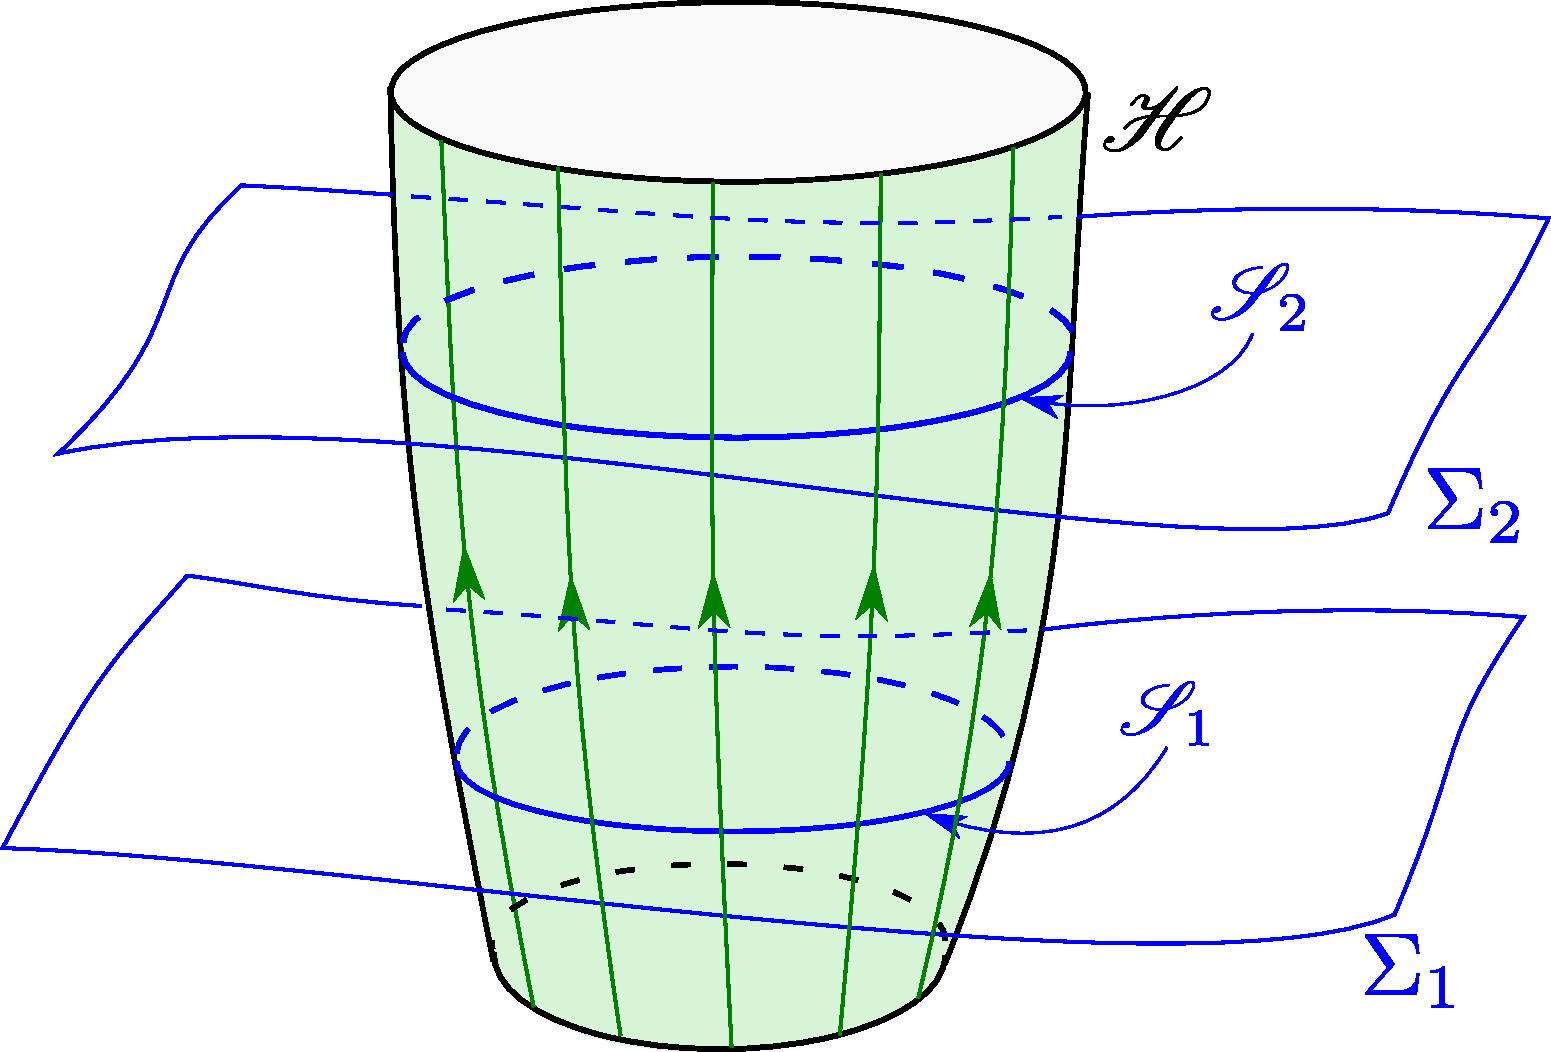
\includegraphics[width=0.6\textwidth]{evo_area_thm_smooth.pdf}}
\caption[]{\label{f:evo:area_thm_smooth} \footnotesize
Cross-sections $\Sp_1$ and $\Sp_2$ induced by the spacelike hypersurfaces $\Sigma_1$
and $\Sigma_2$ in a smooth part of the event horizon $\Hor$,
such that $\Sp_1$ and $\Sp_2$ are intersected by the same null geodesic
generators of $\Hor$ (green curves).}
\end{figure}



\begin{prop}[area theorem \textnormal{(Hawking\index[pers]{Hawking, S.W.} 1971 \cite{Hawki71},
Chru\'sciel\index[pers]{Chrusciel, P.T.@Chru\'sciel, P.T.},
Delay\index[pers]{Delay, E.},
Galloway\index[pers]{Galloway, G.J.} and Howard\index[pers]{Howard, R.} 2001
\cite{ChrusDGH01})}]
\label{p:evo:area_thm}
Let $(\M,\w{g})$ be a $n$-dimensional spacetime containing a black hole
of event horizon $\Hor$ and such that the Ricci tensor $\w{R}$ fulfills the null
convergence condition\index{null!convergence condition}\index{convergence!condition!null --} (\ref{e:neh:null_energy_cond}), i.e.
$\w{R}(\wl, \wl) \geq 0$ for any null vector $\wl$
--- which holds in general relativity if the null energy condition\index{null!energy condition}\index{energy!condition!null --} (\ref{e:neh:null_energy_cond_matter}) is fulfilled.
Let $\Sigma_1$ and $\Sigma_2$ be spacelike hypersurfaces
such that $\Sigma_2$ lies in the causal future of $\Sigma_1$: $\Sigma_2\subset J^+(\Sigma_1)$
(cf. Sec.~\ref{s:glo:causal_struct}). Let $\Sp_1 = \Hor \cap \Sigma_1$
and $\Sp_2 = \Hor\cap\Sigma_2$.
If
\begin{itemize}
\item[(i)] $\Hor$ is smooth between $\Sp_1$ and $\Sp_2$, and $\Sp_1$ and $\Sp_2$
are cross-sections\footnote{If $\Hor$ is smooth between $\Sp_1$ and $\Sp_2$,
it is necessarily a null hypersurface there (Property~\ref{p:glo:prop4} on p.~\pageref{p:glo:prop4}),
so that the concept of cross-section as defined in Sec.~\ref{s:def:spacelike_sections}
makes sense.} of $\Hor$ that are intersected by the same null geodesic generators of $\Hor$
(cf. Fig.~\ref{f:evo:area_thm_smooth})
\end{itemize}
or
\begin{itemize}
\item[(ii)]
the closure of $J^-(\scri^+)\cup \Hor$ in
the conformal manifold $\tilde{\M}\supset\M$ defining $\scri^+$
is included in a globally hyperbolic
region $\mathscr{V}$ of $(\tilde{\M},\tilde{\w{g}})$
and $\Sigma_1$ and $\Sigma_2$ are Cauchy surfaces
of $\mathscr{V}$,
\end{itemize}
then the areas $A(\Sp_1)$ and $A(\Sp_2)$ obey
\be \label{e:evo:AS2_ge_AS1}
    A(\Sp_2) \geq A(\Sp_1) .
\ee
\end{prop}

\begin{figure}
\centerline{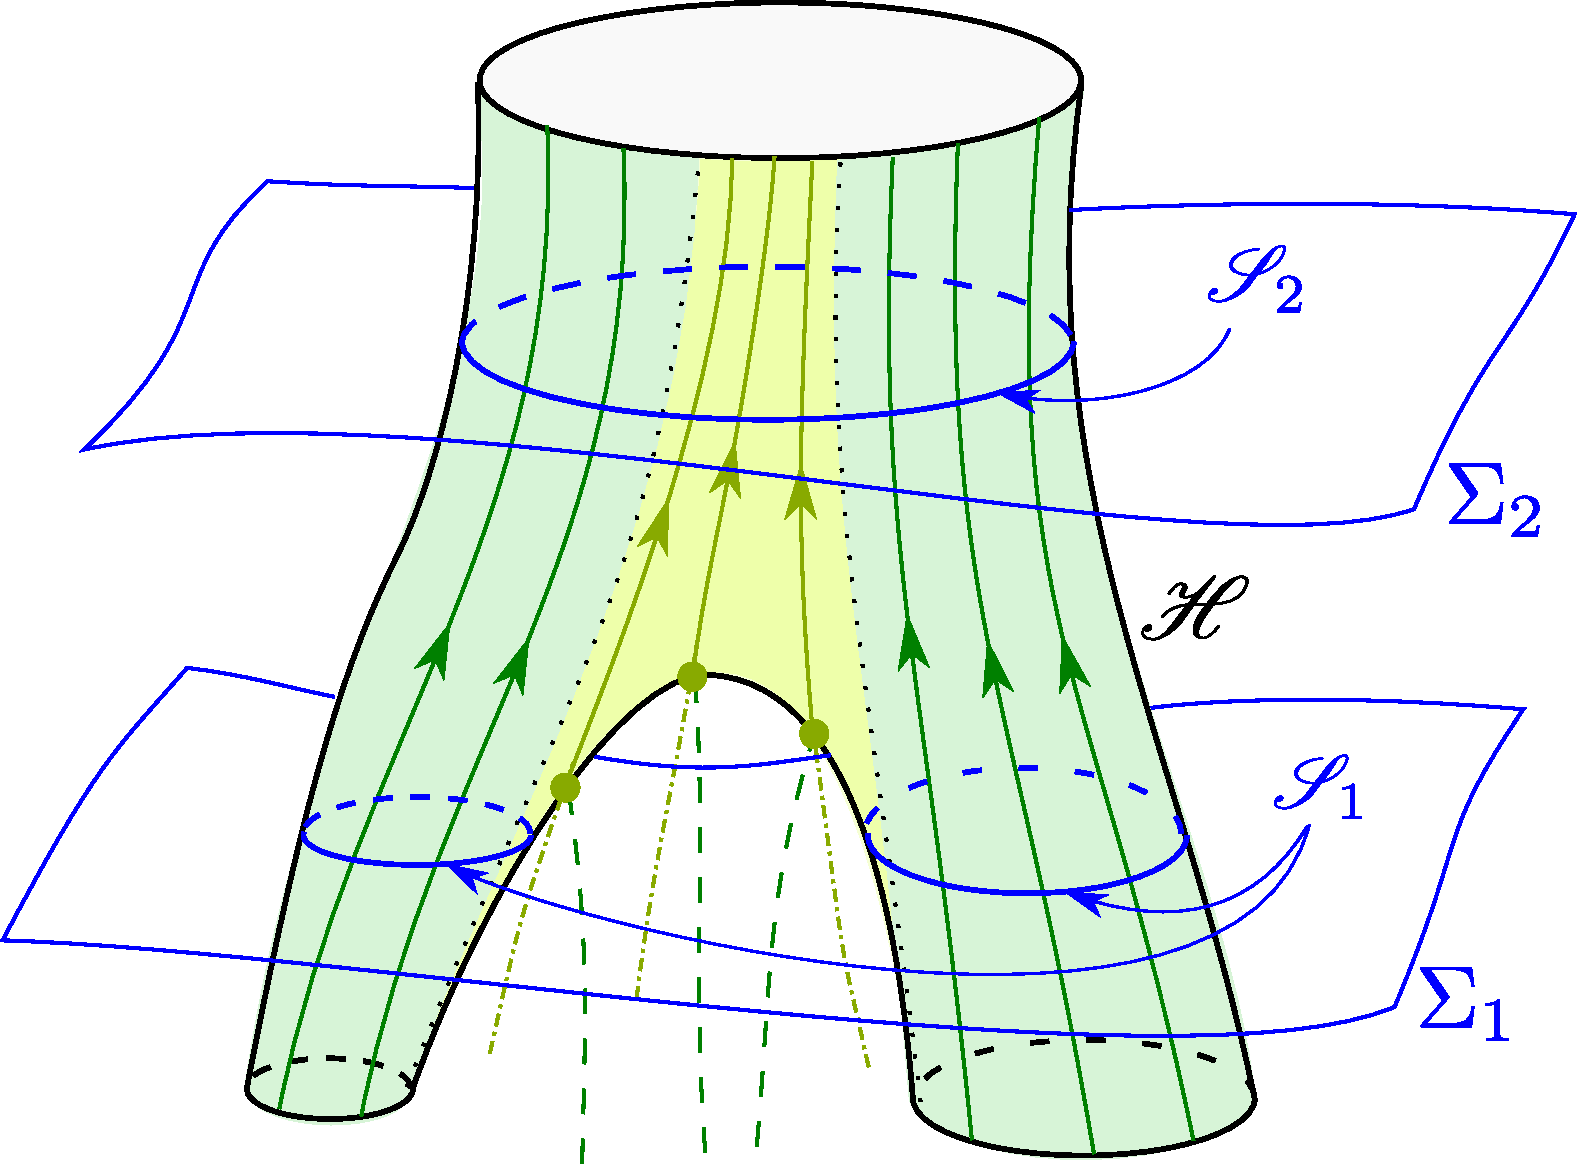
\includegraphics[width=0.6\textwidth]{evo_area_theorem.pdf}}
\caption[]{\label{f:evo:area_theorem} \footnotesize
Surfaces $\Sp_1$ and $\Sp_2$ induced by the spacelike hypersurfaces $\Sigma_1$
and $\Sigma_2$ on the event horizon $\Hor$ corresponding to a black hole merger.
All solid dark green and light green curves are null geodesic generators of $\Hor$.
The light green part of $\Hor$ is generated by null geodesics that
entered $\Hor$ at some caustic points (three of them are indicated as
light green dots); the parts of these geodesics outside $\Hor$ are drawn as
light green dot-dashed curves. The dark green dashed curves depict other null geodesics that
enter $\Hor$ at the same caustic points.}
\end{figure}


\begin{proof}
Let us consider first the case (i) ($\Hor$ smooth between
$\Sp_1$ and $\Sp_2$).
$\Sp_1$ and $\Sp_2$ are then cross-sections of $\Hor$
that are connected by null geodesic generators of $\Hor$
(cf. Fig.~\ref{f:evo:area_thm_smooth}).
One may introduce a 1-parameter foliation $(S_t)_{t\in [0,1]}$ of $\Hor$ by
cross-sections $S_t$ such that $S_0 = \Sp_1$ and $S_1 = \Sp_2$
(cf. the proof of Property~\ref{p:neh:invariance_area} for details, $\lambda$
playing the role of $t$ there). The label $t$
can then be considered as a parameter along the null geodesic generators of $\Hor$
connecting $\Sp_1$ to $\Sp_2$.
Let $\wl = \D\w{x}/\D t$ be the associated tangent vector.
Given that $\Sp_2$ lies in the future of $\Sp_1$, $\wl$ is future-directed.
By the very definition
of the expansion $\theta_{(\wl)}$ along $\wl$ [Eq.~(\ref{e:def:def_expansion})
combined with Eq.~(\ref{e:def:A_sqrt_q})], one has
\[
    \derd{}{t} A(S_t) = \int_{S_t} \theta_{(\wl)} \,  \sqrt{q} \, \D x^2 \cdots \D x^{n-1} ,
\]
where $(x^2, \ldots, x^{n-1})$ is a coordinate system on $S_t$ and $q$ is
the determinant with respect to these coordinates of the metric
induced by $\w{g}$ on $S_t$.
Now, if the null convergence condition holds, Property~\ref{p:evo:positive_expansion} implies
$\theta_{(\wl)} \geq 0$; hence
\[
  \derd{}{t} A(S_t) \geq 0 .
\]
It follows that $t\mapsto A(S_t)$ is a nondecreasing function. Consequently, $A(S_1) \geq A(S_0)$
and Eq.~(\ref{e:evo:AS2_ge_AS1}) holds.

If $\Hor$ is not smooth between $\Sp_1$ and $\Sp_2$, this is due to the crease set\index{crease set},
i.e. the subset of $\Hor$ where new null geodesics enter $\Hor$ (cf. Sec.~\ref{s:glo:properties_H}).
Naively, this reinforces the inequality $A(\Sp_2) > A(\Sp_1)$ since the new geodesics
are generating new parts of $\Hor$ and therefore parts of $\Sp_2$ distinct
from those that can be connected to $\Sp_1$ by null geodesic generators
(cf. Fig.~\ref{f:evo:area_theorem}). More precisely, let us assume (ii) and
let us consider a point $p\in\Sp_1$. Let $\Li$ be the null geodesic
generator of $\Hor$ through $p$. By property~\ref{p:glo:prop3}, $\Li$ stays in $\Hor$ for all its future after $p$. Since $\Sigma_2$ is a Cauchy surface lying in the causal future of $\Sigma_1$, $\Li$
necessarily intersects $\Sigma_2$ at a unique point $q \in \Sigma_2\cap\Hor = \Sp_2$.
Hence every point of $\Sp_1$ is mapped to a point of $\Sp_2$ by a null geodesic generator.
Let $\Sp_2^*$ be the part of $\Sp_2$ covered by this map.
If we assume that the part of $\Hor$ between $\Sp_1$ and $\Sp_2^*$ is smooth,
we may apply (i) to the pair $(\Sp_1, \Sp_2^*)$
and get $A(\Sp_2^*) \geq A(\Sp_1)$. Given that $\Sp_2^* \subset \Sp_2$, one has
$A(\Sp_2) \geq A(\Sp_2^*)$ and (\ref{e:evo:AS2_ge_AS1}) follows.
We refer to the article \cite{ChrusDGH01} for the proof in the case where
$\Hor$ is not assumed smooth between $\Sp_1$ and $\Sp_2^*$ (70 pages!).
\end{proof}

\begin{example}[Oppenheimer-Snyder collapse]
Let us consider the black hole formed by the collapse
of a ball of pressureless matter, as described by the Oppenheimer-Snyder
model studied in Sec.~\ref{s:lem:OS}. Let $\Sp_{\ti}$ be a
cross-section of the event horizon at constant ingoing Eddington-Finkelstein coordinate $\ti$.
The area of $\Sp_{\ti}$ is simply $A = 4\pi r^2$,
where $r$ is the areal radius (cf. Sec.~\ref{s:lem:OS:BH_formation}). Its
evolution can thus be read directly on Fig.~\ref{f:lem:OS:diag_int_EF} (right):
it is increasing from $A = 0$ (at $\ti\simeq 5.6\, m$) to the Schwarzschild
value $A = 16\pi m^2$ (at $\ti\simeq 9.7\, m$). This fully agrees
with the area theorem, given that the null energy condition (\ref{e:neh:null_energy_cond_matter})
is fulfilled by the energy-momentum tensor (\ref{e:lem:T_pressureless}) of the collapsing matter: $\w{T}(\wl,\wl) =  \rho (\w{u}\cdot\wl)^2 \geq 0$ since $\rho \geq 0$.
\end{example}

\begin{example}[Vaidya collapse]
Similarly, we check on Figs.~\ref{f:vai:diag_S0} and \ref{f:vai:diag_S2}
that for the radiation shell collapse studied in Chap.~\ref{s:vai},
the area of cross-sections of the event horizon
at constant ingoing Eddington-Finkelstein coordinate $t$
is increasing towards the future, for $r$ is again the areal radius
[cf. the metric (\ref{e:vai:metric_IEF})]. As we have already noticed in
Sec.~\ref{s:vai:general}, the radiation energy-momentum tensor (\ref{e:vai:ener_mom_tensor})
fulfills the null energy condition, given that $M'(v) \geq 0$ (cf. Fig.~\ref{f:vai:mass_function}).
\end{example}


\begin{hist}
The area theorem has been first established by Stephen Hawking\index[pers]{Hawking, S.W.}
in 1971 \cite{Hawki71} and a detailed proof was given in
Hawking \& Ellis' 1973 textbook (Proposition~9.2.7 in \cite{HawkiE73}).
In 2001, Piotr Chru\'sciel\index[pers]{Chrusciel, P.T.@Chru\'sciel, P.T.},
Erwann Delay\index[pers]{Delay, E.},
Gregory Galloway\index[pers]{Galloway, G.J.} and Ralph Howard\index[pers]{Howard, R.}
\cite{ChrusDGH01} pointed out that the Hawking \& Ellis proof is
valid only for $\Hor$ piecewise smooth (cf. the
discussion in Sec.~3.5.1 of Chru\'sciel's textbook \cite{Chrus20}); they constructed
a new proof that does not assume the smoothness of $\Hor$.
\end{hist}

\subsection{A second law?}

Basically the area theorem~\ref{p:evo:area_thm} states that
the area of cross-sections of a black hole event horizon
cannot decrease from the past to the future.
By its irreversible character, this property bears some resemblance
with the second law of thermodynamics.
By itself, this is of course not sufficient to identify the black hole area
with some entropy (any nondecaying physical quantity has not to be an entropy!).
However, we have seen in Sec.~\ref{s:evo:a_first_law_question} that the
candidate $T\D S$ term for a possible first law could be $\kappa/(8\pi)\D A$.
It is thus tempting to identify $A$ with some entropy $S$, up to some
constant factor $\alpha$. Then the temperature $T$ would be $\kappa/(8\pi\alpha)$:
\be \label{e:evo:identif_S_T}
    S = \alpha A \qand T = \frac{1}{8 \pi\alpha}\, \kappa ,
\ee
so that we get $T\D S = \kappa/(8\pi)\D A$, making
the mass variation formula (\ref{e:evo:mass_variation}) look pretty much like
the first law of thermodynamics.

%%%%%%%%%%%%%%%%%%%%%%%%%%%%%%%%%%%%%%%%%%%%%%%%%%%%%%%%%%%%%%%%%%%%%%%%%%%%%%%

\section{The other laws of thermodynamics}

\subsection{Zeroth law}

We have already established a so-called \emph{zeroth law of black hole dynamics}
in Chap.~\ref{s:neh}, namely Property~\ref{p:neh:zeroth_law}, which states that
if the null dominance condition is fulfilled, the surface gravity
$\kappa$ of a Killing horizon is constant. Now, by Properties~\ref{p:sta:H_Killing_hor_xi_null}
and \ref{p:sta:strong_rigidity_thm}, (a connected component of) the event horizon
of a stationary black hole must be a Killing horizon. Hence, we may extend
the zeroth law to black holes\index{zeroth law!of BH dynamics}:

\begin{prop}[zeroth law of black hole dynamics]
Let $(\M,\w{g})$ be a stationary spacetime of dimension $n\geq 4$ containing a black
hole. Let $\Hor$ be a connected component of the black hole event horizon.
If the null dominance condition\index{null!dominance condition}\index{dominance!null -- condition} (\ref{e:neh:null_dominant_cond})
is fulfilled on $\Hor$  --- which is guaranteed in general relativity
if the null dominant energy condition\index{null!dominant energy condition}\index{energy!condition!null dominant --} (\ref{e:neh:null_dominant_cond_T}) holds on $\Hor$ ---
and under the hypotheses of
Property~\ref{p:sta:strong_rigidity_thm} if $\Hor$ is rotating
(i.e. if the stationary Killing vector $\w{\xi}$ is spacelike on some parts
of $\Hor$), then the surface gravity $\kappa$ is constant over $\Hor$.
\end{prop}

Given that a black hole ``in equilibrium'' is modeled by a black hole in
a stationary spacetime,
this property bears a strong resemblance with
the \emph{zeroth law of thermodynamics}\index{zeroth law!of thermodynamics}, which states that the temperature of a body in equilibrium
is uniform over the entire body.
This strengthens the interpretation of the surface gravity
$\kappa$ as the temperature $T$ (up to some factor) performed in
Eq.~(\ref{e:evo:identif_S_T}).


\subsection{What about the third law?}

The classical Nernst formulation of the \emph{third law of thermodynamics}\index{third law!of thermodynamics}
states that the entropy of a system must approach zero (or a universal constant)
as its temperature tends to zero. In this form and with the identification (\ref{e:evo:identif_S_T}), it certainly does not hold for black holes, because
well known extremal black holes, which have $\kappa=0$, have a non-vanishing area. For
instance, the area of the extremal Kerr black hole\index{extremal!Kerr spacetime}\index{Kerr!extremal -- spacetime} of mass $m$ (Chap.~\ref{s:exk}) is
$A = 8\pi m^2$ (take the limit $a\to m$ in Eq.~(\ref{e:ker:A_a_m})),
which neither zero, nor a universal constant. Similarly, the area of
the extremal Reissner-Nordström black hole\index{Reissner-Nordström!black hole!extremal --}\index{extremal!Reissner-Nordström!black hole} of mass $m$ is $A = 4\pi m^2$
(this is immediate from the metric (\ref{e:loc:metric_ERN}) below).
Another formulation of the third law of thermodynamics states that it is impossible to bring any
system to a zero temperature by a finite number of operations. This was the formulation adopted
for black holes, as a conjecture, by Bardeen, Carter and Hawking in 1973 \cite{BardeCH73}.
It was then reformulated, with a tentative proof, by Israel in 1986 \cite{Israe86b}, as
\begin{quote}
No continuous process in which the energy-momentum tensor of accreted matter remains
bounded and satisfies the weak energy
condition\index{weak!energy condition}\index{energy!condition!weak --} in a neighborhood of the apparent
horizon can reduce the surface gravity of a black hole to zero
within a finite advanced time.
\end{quote}
However, as pointed out recently by Kehle\index[pers]{Kehle, C.} and Unger\index[pers]{Unger, R.} \cite{KehleU23}, Israel's proof
is restricted to the case where outermost trapped surfaces evolve smoothly, while, as we shall discuss in Chap.~\ref{s:loc},
their evolution generically presents discontinuous jumps, even if the spacetime
and all the matter fields remain perfectly smooth. In particular, Kehle and Unger \cite{KehleU23} have exhibited
a spacetime where the collapse of a $C^k$-regular charged scalar field (obeying the dominant, and hence the weak, energy condition) turns a (piece of) Schwarzschild black hole
into an extremal Reissner-Nordström black hole within a finite advanced time\footnote{As shown
in Sec.~5.5.6 of Poisson's textbook \cite{Poiss04}, this cannot happen with a charged null dust
(i.e. a charged generalization of Vaidya collapse discussed in Chap.~\ref{s:vai}) that obeys
the weak energy condition.}.

From an astrophysical point of view, Bardeen\index[pers]{Bardeen, J.M.} has shown in 1970 \cite{Barde70a}
that a Schwarzschild black hole
of mass $m_0$ ($\kappa = 1/(4m_0) > 0$, Eq.~(\ref{e:def:kappa_Schw_hor}))
can in principle be spun up to an extremal Kerr black hole
($\kappa = 0$)
by accreting matter from the
innermost stable circular orbit\index{innermost!stable circular orbit}\index{circular!orbit!innermost stable --}
(ISCO, cf. Sec.~\ref{s:gek:circ_orb_stab}) by a total rest-mass amount of
$\simeq 1.86\, m_0$; the mass of the final black hole is then $m \simeq 2.45\, m_0$.
However, if one assumes that the matter comes from an accretion disk\index{accretion!disk}
terminating at the ISCO and
one takes into account the electromagnetic emission of the disk, the extremal Kerr state
cannot be achieved. The reason is that a substantial part of the emitted photons carry a negative angular momentum $\ell$ and
the black hole absorption cross-section for photons with $\ell<0$ is larger than for those with
$\ell>0$. This appears clearly on the shadow picture of Fig.~\ref{f:gik:shadow_a95},
where the part $\alpha>0$, which is due to photons
with $\ell < 0$ (cf. Eq.~\ref{e:gik:shadow_param_eq_alpha}), is much larger than the part $\alpha<0$
corresponding to $\ell > 0$. Consequently, the black hole absorbs more photons with $\ell < 0$
than with $\ell>0$; this diminishes the increase of the black hole spin $a$ resulting form the accretion of  matter from the disk (which has a positive angular momentum). Thorne\index[pers]{Thorne, K.S.} has shown in 1974 \cite{Thorn74} that the balance between the two processes leads to a final reduced spin $a \simeq 0.998 \, m$, quite insensitive to the details
of the emission mechanism in the accretion disk. This is close to, but strictly lower than, the critical
value $a = m$ that would have yield a zero surface gravity. Hence, in this respect, we can say that
astrophysical black holes absorbing matter from an accretion disk obey a kind of third law of thermodynamics.
But this does not appear to arise from some fundamental properties of black holes; it rather results from the properties of their environment.

It must be stressed that in the field of standard thermodynamics as well, the third law has not the same fundamental status as the other laws.
In particular it can be violated by some rather simple systems (see Ref.~\cite{Wald97} for a discussion and an example involving a boson (or fermion) gas confined to a circular ring).

For all the above reasons, we shall no longer discuss the third law here.

%%%%%%%%%%%%%%%%%%%%%%%%%%%%%%%%%%%%%%%%%%%%%%%%%%%%%%%%%%%%%%%%%%%%%%%%%%%%%%%

\section{Black hole thermodynamics}

\subsection{The three laws}

\subsection{Hawking radiation and Bekenstein-Hawking entropy}

\subsection{The generalized second law}

